% Practice Test 05 — Florida Edition
% Questions: 30 (25 MC + 5 SA)
% Generated by scripts/generate_practice_tests.py

\begin{practiceQuestion}{1-3-q04}{mc}
\begin{questionText}
Bananas cost a fixed price per pound. The table shows the relationship. What is $k$?

\begin{center}
\begin{tabular}{|c|c|}
\hline \textbf{Pounds} & \textbf{Cost (\$)} \\ \hline $2$ & $\$1.30$ \\ $5$ & $\$3.25$ \\ $8$ & $\$5.20$ \\ \hline
\end{tabular}
\end{center}
\end{questionText}
\choiceA{$\$0.55$ per pound}
\choiceB{$\$0.65$ per pound}
\choiceC{$\$1.30$ per pound}
\choiceD{$\$1.54$ per pound}
\correctAnswer{B}
\explanation{$k = \frac{1.30}{2} = 0.65$. Check: $\frac{3.25}{5} = 0.65$ and $\frac{5.20}{8} = 0.65$. Bananas cost $\$0.65$ per pound.}
\end{practiceQuestion}

\begin{practiceQuestion}{1-6-q15}{mc}
\begin{questionText}
A car uses $3$ gallons of gas every $87$ miles. How many gallons does it need for a $435$-mile trip?
\end{questionText}
\choiceA{$10$}
\choiceB{$12$}
\choiceC{$15$}
\choiceD{$18$}
\correctAnswer{C}
\explanation{$\frac{3}{87} = \frac{x}{435}$. Cross-multiply: $87x = 1{,}305$, so $x = 15$ gallons.}
\end{practiceQuestion}

\begin{practiceQuestion}{2-1-q06}{mc}
\begin{questionText}
$14$ is what percent of $56$?
\end{questionText}
\choiceA{$14\%$}
\choiceB{$20\%$}
\choiceC{$25\%$}
\choiceD{$28\%$}
\correctAnswer{C}
\explanation{Divide the part by the whole: $14 \div 56 = 0.25 = 25\%$.}
\end{practiceQuestion}

\begin{practiceQuestion}{2-2-q24}{sa}
\begin{questionText}
$156$ is $120\%$ of what number?
\end{questionText}
\correctAnswer{$130$}
\explanation{$\frac{156}{w} = \frac{120}{100}$. Cross-multiply: $120w = 15{,}600$. Divide: $w = 130$.}
\end{practiceQuestion}

\begin{practiceQuestion}{2-6-q27}{gmc}
\begin{questionText}
The table below compares two savings plans. Which plan earns more interest?

\begin{center}
\begin{tabular}{|l|c|c|c|}
\hline
 & \textbf{Principal} & \textbf{Rate} & \textbf{Time} \\
\hline
Plan A & $\$2{,}000$ & $3\%$ & $4$ years \\
\hline
Plan B & $\$1{,}500$ & $4\%$ & $4$ years \\
\hline
\end{tabular}
\end{center}
\end{questionText}
\choiceA{Plan A by $\$240$}
\choiceB{Plan A by $\$0$}
\choiceC{Plan B by $\$240$}
\choiceD{They earn the same}
\correctAnswer{D}
\explanation{Plan A: $2{,}000 \times 0.03 \times 4 = \$240$. Plan B: $1{,}500 \times 0.04 \times 4 = \$240$. Both earn $\$240$.}
\end{practiceQuestion}

\begin{practiceQuestion}{2-7-q16}{mc}
\begin{questionText}
An estimate has a percent error of $0\%$. What does this mean?
\end{questionText}
\choiceA{The estimate was very close}
\choiceB{The estimate was exactly correct}
\choiceC{The actual value was $0$}
\choiceD{There was no actual value to compare}
\correctAnswer{B}
\explanation{A $0\%$ percent error means the estimated value equals the actual value exactly.}
\end{practiceQuestion}

\begin{practiceQuestion}{3-2-q10}{mc}
\begin{questionText}
What is $0 + (-7)$?
\end{questionText}
\choiceA{$7$}
\choiceB{$0$}
\choiceC{$-7$}
\choiceD{$-14$}
\correctAnswer{C}
\explanation{Adding $0$ to any number gives that number. $0 + (-7) = -7$.}
\end{practiceQuestion}

\begin{practiceQuestion}{3-3-q28}{gmc}
\begin{questionText}
The table shows daily high temperatures for a city.

\begin{center}
\begin{tabular}{|c|c|}
\hline
\textbf{Day} & \textbf{High Temp (°F)} \\
\hline
Monday & $-3$ \\
\hline
Tuesday & $8$ \\
\hline
Wednesday & $-5$ \\
\hline
\end{tabular}
\end{center}

What is the difference between Tuesday's and Wednesday's temperatures?
\end{questionText}
\choiceA{$3°$F}
\choiceB{$-3°$F}
\choiceC{$13°$F}
\choiceD{$-13°$F}
\correctAnswer{C}
\explanation{$8 - (-5) = 8 + 5 = 13°$F.}
\end{practiceQuestion}

\begin{practiceQuestion}{4-4-q13}{mc}
\begin{questionText}
Which expression is equivalent to $3(4x - 7)$?
\end{questionText}
\choiceA{$12x - 7$}
\choiceB{$12x + 21$}
\choiceC{$12x - 21$}
\choiceD{$7x - 21$}
\correctAnswer{C}
\explanation{Expand to verify: $3 \times 4x = 12x$ and $3 \times (-7) = -21$. So $3(4x - 7) = 12x - 21$.}
\end{practiceQuestion}

\begin{practiceQuestion}{4-5-q01}{mc}
\begin{questionText}
Simplify $(3x + 5) + (2x + 4)$.
\end{questionText}
\choiceA{$5x + 9$}
\choiceB{$6x + 9$}
\choiceC{$5x + 1$}
\choiceD{$5x - 9$}
\correctAnswer{A}
\explanation{Remove parentheses and combine: $(3x + 2x) + (5 + 4) = 5x + 9$.}
\end{practiceQuestion}

\begin{practiceQuestion}{5-3-q03}{mc}
\begin{questionText}
What is the first step to solve $5(x + 2) = 35$ using the ``divide first'' method?
\end{questionText}
\choiceA{Subtract $2$ from both sides}
\choiceB{Distribute $5$ to get $5x + 10 = 35$}
\choiceC{Divide both sides by $5$}
\choiceD{Subtract $5$ from both sides}
\correctAnswer{C}
\explanation{The ``divide first'' method divides both sides by $5$: $x + 2 = 7$.}
\end{practiceQuestion}

\begin{practiceQuestion}{5-4-q08}{mc}
\begin{questionText}
A recipe calls for $\dfrac{3}{4}$ cup of sugar per batch. You already used $\dfrac{1}{2}$ cup. You have $2\dfrac{3}{4}$ cups total. The equation $\dfrac{3}{4}b + \dfrac{1}{2} = 2\dfrac{3}{4}$ finds how many more batches $b$ you can make. What is $b$?
\end{questionText}
\choiceA{$b = 3$}
\choiceB{$b = 4$}
\choiceC{$b = 2$}
\choiceD{$b = 3\dfrac{2}{3}$}
\correctAnswer{A}
\explanation{Subtract $\frac{1}{2}$: $\frac{3}{4}b = 2\frac{1}{4} = \frac{9}{4}$. Multiply by $\frac{4}{3}$: $b = \frac{9}{4} \times \frac{4}{3} = 3$.}
\end{practiceQuestion}

\begin{practiceQuestion}{5-5-q18}{mc}
\begin{questionText}
Solve $-x + 9 \leq 15$.
\end{questionText}
\choiceA{$x \leq -6$}
\choiceB{$x \geq 6$}
\choiceC{$x \geq -6$}
\choiceD{$x \leq 6$}
\correctAnswer{C}
\explanation{Subtract $9$: $-x \leq 6$. Multiply by $-1$ and flip: $x \geq -6$.}
\end{practiceQuestion}

\begin{practiceQuestion}{5-6-q29}{gsa}
\begin{questionText}
Solve $-3x + 9 > 0$. Then graph the solution on the number line below by describing the circle type and shading direction.

\begin{center}
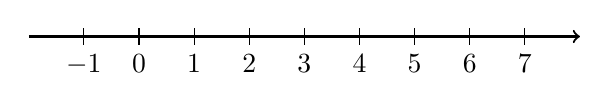
\begin{tikzpicture}[scale=0.7]
  \draw[thick,->] (-2,0) -- (8,0);
  \foreach \x in {-1,...,7} \draw (\x,0.15) -- (\x,-0.15) node[below] {$\x$};
\end{tikzpicture}
\end{center}
\end{questionText}
\correctAnswer{$x < 3$; open circle at $3$, shade left}
\explanation{Subtract $9$: $-3x > -9$. Divide by $-3$ and flip: $x < 3$. Open circle at $3$, shade left.}
\end{practiceQuestion}

\begin{practiceQuestion}{6-2-q17}{mc}
\begin{questionText}
A map uses $1$ cm $= 60$ km. You redraw it at $1$ cm $= 20$ km. A triangle on the original has an area of $4$ cm$^2$. What is its area on the new map?
\end{questionText}
\choiceA{$12$ cm$^2$}
\choiceB{$16$ cm$^2$}
\choiceC{$36$ cm$^2$}
\choiceD{$48$ cm$^2$}
\correctAnswer{C}
\explanation{Scale ratio: $\frac{60}{20} = 3$. Area scales by $3^2 = 9$. New area: $4 \times 9 = 36$ cm$^2$.}
\end{practiceQuestion}

\begin{practiceQuestion}{6-4-q08}{mc}
\begin{questionText}
You know two angles ($50°$ and $70°$) and the side between them is $8$ cm. What triangle condition is this?
\end{questionText}
\choiceA{SSS}
\choiceB{SAS}
\choiceC{ASA}
\choiceD{AAS}
\correctAnswer{C}
\explanation{Two angles and the included side is the ASA (Angle-Side-Angle) condition.}
\end{practiceQuestion}

\begin{practiceQuestion}{6-5-q08}{mc}
\begin{questionText}
A cylinder is sliced with a vertical cut through its center, perpendicular to the base. What shape is the cross-section?
\end{questionText}
\choiceA{Circle}
\choiceB{Rectangle}
\choiceC{Oval}
\choiceD{Triangle}
\correctAnswer{B}
\explanation{A vertical cut through the center of a cylinder produces a rectangle. The width equals the diameter and the height equals the cylinder's height.}
\end{practiceQuestion}

\begin{practiceQuestion}{6-6-q25}{sa}
\begin{questionText}
Two lines intersect. One of the four angles is $(4x + 20)°$. Its adjacent angle is $(6x - 10)°$. Find the value of $x$.
\end{questionText}
\correctAnswer{$17$}
\explanation{Adjacent angles at an intersection are supplementary: $4x + 20 + 6x - 10 = 180$. Combine: $10x + 10 = 180$. Solve: $10x = 170$, $x = 17$.}
\end{practiceQuestion}

\begin{practiceQuestion}{7-1-q02}{mc}
\begin{questionText}
A circle has a radius of $6$ cm. What is its diameter?
\end{questionText}
\choiceA{$3$ cm}
\choiceB{$6$ cm}
\choiceC{$12$ cm}
\choiceD{$18$ cm}
\correctAnswer{C}
\explanation{The diameter is twice the radius: $d = 2r = 2 \times 6 = 12$ cm.}
\end{practiceQuestion}

\begin{practiceQuestion}{7-5-q10}{mc}
\begin{questionText}
A cube has a surface area of $54$ cm$^2$. What is the area of one face?
\end{questionText}
\choiceA{$6$ cm$^2$}
\choiceB{$9$ cm$^2$}
\choiceC{$18$ cm$^2$}
\choiceD{$27$ cm$^2$}
\correctAnswer{B}
\explanation{A cube has $6$ identical faces. Area of one face $= 54 \div 6 = 9$ cm$^2$.}
\end{practiceQuestion}

\begin{practiceQuestion}{7-6-q10}{mc}
\begin{questionText}
A rectangular prism has a base area of $24$ cm$^2$ and a height of $7$ cm. What is its volume?
\end{questionText}
\choiceA{$31$ cm$^3$}
\choiceB{$168$ cm$^3$}
\choiceC{$336$ cm$^3$}
\choiceD{$17$ cm$^3$}
\correctAnswer{B}
\explanation{$V = Bh = 24 \times 7 = 168$ cm$^3$.}
\end{practiceQuestion}

\begin{practiceQuestion}{7-7-q18}{mc}
\begin{questionText}
If you double the height of a cylinder but keep the radius the same, what happens to the volume?
\end{questionText}
\choiceA{It stays the same}
\choiceB{It doubles}
\choiceC{It quadruples}
\choiceD{It increases by a factor of $8$}
\correctAnswer{B}
\explanation{$V = \pi r^2 h$. If $h$ becomes $2h$, then $V = \pi r^2(2h) = 2\pi r^2 h$. The volume doubles.}
\end{practiceQuestion}

\begin{practiceQuestion}{8-1-q11}{mc}
\begin{questionText}
A survey of $200$ randomly selected adults found that $60\%$ prefer coffee over tea. If the city has $50{,}000$ adults, about how many prefer coffee?
\end{questionText}
\choiceA{$12{,}000$}
\choiceB{$20{,}000$}
\choiceC{$30{,}000$}
\choiceD{$60{,}000$}
\correctAnswer{C}
\explanation{$60\%$ of $50{,}000 = 0.60 \times 50{,}000 = 30{,}000$.}
\end{practiceQuestion}

\begin{practiceQuestion}{8-3-q08}{mc}
\begin{questionText}
The dot plots for two classes overlap significantly. The difference in their means is $2$ points, and both have a MAD of $6$. What can you conclude?
\end{questionText}
\choiceA{The classes are very different}
\choiceB{The difference in means is meaningful}
\choiceC{The difference in means is small relative to the variability}
\choiceD{You cannot compare the classes}
\correctAnswer{C}
\explanation{The difference ($2$) is much smaller than the MAD ($6$), so the difference is not very meaningful — there is a lot of overlap.}
\end{practiceQuestion}

\begin{practiceQuestion}{8-4-q30}{gsa}
\begin{questionText}
The table shows test scores for two science classes.

\begin{center}
\begin{tabular}{|l|c|c|c|c|c|c|c|c|c|c|}
\hline
\textbf{Class A} & $60$ & $65$ & $70$ & $75$ & $80$ & $85$ & $90$ & $95$ & & \\
\hline
\textbf{Class B} & $72$ & $74$ & $76$ & $78$ & $80$ & $82$ & $84$ & $86$ & & \\
\hline
\end{tabular}
\end{center}

Find the mean, median, and range for each class. Which class performed more consistently?
\end{questionText}
\correctAnswer{Both means $= 77.5$; both medians $= 77.5$; Class A range $= 35$, Class B range $= 14$. Class B is more consistent.}
\explanation{Class A: mean $= \frac{620}{8} = 77.5$, median $= \frac{75+80}{2} = 77.5$, range $= 95 - 60 = 35$. Class B: mean $= \frac{632}{8} = 79$, median $= \frac{78+80}{2} = 79$, range $= 86 - 72 = 14$. Class B has a much smaller range, so its scores are more consistent.}
\end{practiceQuestion}

\begin{practiceQuestion}{8-5-q02}{mc}
\begin{questionText}
Which of the following is true about the leaves in a stem-and-leaf plot?
\end{questionText}
\choiceA{Leaves are listed in random order}
\choiceB{Leaves are listed in order from least to greatest}
\choiceC{Each leaf represents the tens digit}
\choiceD{Leaves are always single digits from $1$ to $9$}
\correctAnswer{B}
\explanation{Leaves must be arranged in order from least to greatest so the data is easy to read.}
\end{practiceQuestion}

\begin{practiceQuestion}{8-6-q26}{gmc}
\begin{questionText}
The circle graph shows how $400$ students get to school.

\begin{center}
\begin{tikzpicture}[scale=1.2]
  % Bus 40%, Walk 25%, Car 20%, Bike 15%
  \fill[funBlue!60] (0,0) -- (0,1.5) arc (90:90-144:1.5) -- cycle;
  \fill[funGreen!60] (0,0) -- (90-144:1.5) arc (90-144:90-144-90:1.5) -- cycle;
  \fill[funOrange!60] (0,0) -- (90-144-90:1.5) arc (90-144-90:90-144-90-72:1.5) -- cycle;
  \fill[funRed!40] (0,0) -- (90-144-90-72:1.5) arc (90-144-90-72:90:1.5) -- cycle;
  \draw (0,0) circle (1.5);
  \node[font=\small\bfseries] at (60:1) {Bus};
  \node[font=\tiny] at (60:0.65) {$40\%$};
  \node[font=\small\bfseries] at (-30:1) {Walk};
  \node[font=\tiny] at (-30:0.65) {$25\%$};
  \node[font=\small\bfseries] at (-110:1) {Car};
  \node[font=\tiny] at (-110:0.65) {$20\%$};
  \node[font=\small\bfseries] at (170:1) {Bike};
  \node[font=\tiny] at (170:0.65) {$15\%$};
\end{tikzpicture}
\end{center}

How many students walk to school?
\end{questionText}
\choiceA{$25$}
\choiceB{$60$}
\choiceC{$80$}
\choiceD{$100$}
\correctAnswer{D}
\explanation{$25\%$ of $400 = 0.25 \times 400 = 100$ students.}
\end{practiceQuestion}

\begin{practiceQuestion}{9-4-q24}{sa}
\begin{questionText}
Create a non-uniform probability model for a spinner with $3$ sections (A, B, C) where A is twice as likely as B, and C has the same probability as B. Write the probability of each section.
\end{questionText}
\correctAnswer{$P(A) = \frac{1}{2}$, $P(B) = \frac{1}{4}$, $P(C) = \frac{1}{4}$}
\explanation{Let $P(B) = x$. Then $P(A) = 2x$ and $P(C) = x$. Total: $2x + x + x = 4x = 1$, so $x = \frac{1}{4}$. $P(A) = \frac{1}{2}$, $P(B) = P(C) = \frac{1}{4}$.}
\end{practiceQuestion}

\begin{practiceQuestion}{9-6-q13}{mc}
\begin{questionText}
Two coins are flipped. What is the probability of getting at least one head?
\end{questionText}
\choiceA{$\frac{1}{4}$}
\choiceB{$\frac{1}{2}$}
\choiceC{$\frac{3}{4}$}
\choiceD{$1$}
\correctAnswer{C}
\explanation{At least one head: HH, HT, TH — that is $3$ out of $4$. $P = \frac{3}{4}$. Or: $1 - P(\text{no heads}) = 1 - \frac{1}{4} = \frac{3}{4}$.}
\end{practiceQuestion}

\begin{practiceQuestion}{9-7-q11}{mc}
\begin{questionText}
A bag has $3$ red and $7$ blue marbles. To simulate drawing one marble, you could use random digits $0$--$9$. Which digits would represent red?
\end{questionText}
\choiceA{$0, 1, 2$}
\choiceB{$0, 1, 2, 3$}
\choiceC{$0, 1, 2, 3, 4, 5, 6$}
\choiceD{$7, 8, 9$}
\correctAnswer{A}
\explanation{Red has a $\frac{3}{10}$ probability. Using $3$ digits ($0, 1, 2$) out of $10$ gives $\frac{3}{10} = 30\%$.}
\end{practiceQuestion}
